\chapter{Modelado Empírico de Perfiles de Transporte}\label{sec:NLS}
\section{Introducción}
Como se mencionó en la Sección \ref{sec:performanceparameters}, los perfiles de transporte otorgan una visión amplia del desempeño de un sistema de membranas para transportar una determinada especie. Los perfiles pueden analizarse rápidamente de manera gráfica, pero la principal desventaja de esta estrategia reside en que dos sistemas similares darán lugar a perfiles de transporte también similares, en cuyo caso, el análisis meramente gráfico no permitirá elucidar de manera objetiva las diferencias sutiles en el desempeño, a las que pueda haber lugar. Una alternativa sistemática de analizar los perfiles de transporte es a través de su modelamiento con ecuaciones empíricas. En este caso, se desea que los modelos escogidos describan apropiadamente los datos experimentales, y que los parámetros de las ecuaciones estén relacionados de alguna manera con los indicadores de desempeño del sistema. \index{Perfiles de transporte!Modelado de}


\citet{RODRIGUEZDESANMIGUEL2014} reportaron una ecuación que permite modelar los cambios de concentración de iones cromo en las disoluciones de alimentación y recuperación, en un proceso de transporte facilitado usando una PIM. Se encontró que los parámetros ajustables son de utilidad para optimizar los sistemas cuando son usados como variables respuesta en un diseño experimental (ver Sección \ref{sec:DoE}). Los parámetros se obtienen usando regresión no lineal por mínimos cuadrados (NLS)\acused{NLS}. En el reporte, las fracciones de ión cromo son ajustadas en función del tiempo $t$, con la siguiente ecuación:
\begin{equation}
    \Phi_i = A_ie^{-t/d_i} + y_{0,i}
\end{equation}
donde $\Phi_i$ son las fracciones de cromo en las disolucies de alimentación ($i = ali$) y recuperación ($i = rec$). $A_i$, $d_i$, y $y_{0,i}$ son los parámetros ajustables. $A_i$ se relaciona con el intercepto en el eje de las ordenadas del perfil de transporte, $d_i$ está relacionado con que tan marcado es el cambio en las fracciones en función del tiempo, y $y_{0,i}$ se relaciona con el valor límite que se alcanza en cada fase a largos tiempos de transporte.

Los parámetros ajustables en un mismo sistema difieren dependiendo de si se modela la fracción en la disolución de alimentación o en la de recuperación y esto impide que puedan ser promediados entre si. Para usar los parámetros los autores sugirieron dos funciones que denominaron $G_{feed}$ y $G_{strip}$. Estas funciones combinan los parámetros de regresión para cada disolución de una manera similar a como lo haría una función de deseabilidad.
\begin{equation}
    G_{feed}=\frac{1}{y_{0,ali}d_{ali}};\qquad G_{strip}=\frac{y_{0,rec}}{d_{rec}}
\end{equation}
La maximización de $G_{feed}$ y $G_{strip}$ por medio de un diseño experimental, permitió la obtención de las mejores condiciones para el proceso de transporte bajo estudio \citep{RODRIGUEZDESANMIGUEL2014}. Una propuesta similar de modelado empírico de procesos de transporte se utilizó en el presente trabajo, y su descripción se hace en la siguiente sección.

\section{Nueva propuesta}
%JCCA: ¿Por qué no buscar modelar la cinética de tranasporte, en lugar de utilizar un modelo empírico como este? Revisa, por ejemplo, Biophysical Chemistry, 35 (1990) 85-95 Kinetic model for membrane transport 1. Effects of membrane volume and partitioning kinetics.
%CAPC Holy damn shit! fuck! Admitamos inferioridad intelectual y tratemos de vender nuestra mierda mediocre :c
Modelar la cinética del proceso de transporte considerando la dinámica de todos los pasos involucrados permite estudiar de manera rigurosa el comportamiento del sistema, sin necesidad de recurrir a modelos empíricos y en algunos casos, haciendo un mínimo número de asunciones muy razonables. Estos modelos tienen la belleza de reflejar adecuadamente la realidad de los fenómenos bajo estudio \citep{MAKINO199085}. Sin embargo, el precio a pagar por cualidades tan apetecibles es con frecuencia una elevada complejidad matemática en el modelo, lo cual puede dificultar el avance de una investigación en la que se buscan las mejores condiciones para el transporte selectivo de una especie a través de una membrana. Acá es donde entran a jugar los modelos empíricos que por lo general son mucho más simples y requieren una cantidad mucho menor de información del sistema bajo estudio. Estos modelos empíricos son muy prácticos y pueden usarse en procesos de optimización, gracias a que la obtención de sus parámetros es con regularidad muy fácil y rápida. 

En el desarrollo del presente trabajo se observó que las fracciones de las especies en función del tiempo se comportan de manera similar a las cinéticas enzimáticas tipo Michaelis-Menten \citep{Johnson2011}, o a las isotermas de adsorción tipo Langmuir \citep{Atkins}. Esto sugiere que los perfiles de transporte pueden ser modelados con ecuaciones similares a las utilizadas en los fenómenos mencionados. Las ecuaciones a las que se ajustaron los perfiles de transporte para las disoluciones de alimentación y de recuperación, como fracción transportada en función del tiempo ($\Phi_{ali}(t)$ y $\Phi_{rec}(t)$, respectivamente) se muestran a continuación.

\begin{equation}\label{eq:NLSCRIS}
    \Phi_{ali}=1-\frac{\alpha_{ali} t^\kappa}{\beta_{ali}^{-1}+t^\kappa};\qquad\Phi_{rec}=\frac{\alpha_{rec} t^\kappa}{\beta_{rec}^{-1}+t^\kappa}
\end{equation}

donde $\alpha_i$ y $\beta_i$ se relacionan con los valores máximos transportados y la rapidez a la que ocurre dicho proceso, respectivamente. Valores altos de $\alpha$ y de $\beta$ implican procesos de transporte más eficientes y más veloces, respectivamente. $\kappa$ es igual a uno en la mayoría de los casos y es usado para mejorar el ajuste de las ecuaciones propuestas dado que algunos sistemas pueden mostrar algo de excentricidad que debe ser corregida en la ecuación empírica. Este parámetro $\kappa$ no es hallado por \ac{NLS} sino que debe definirse para cada conjunto de experimentos. Para que los valores de $\alpha$ y $\beta$ de dos sistemas puedan ser comparados entre sí, debe usarse el mismo valor de $\kappa$ en la regresión no lineal.


Para ilustrar la variación en los perfiles de transporte con los parámetros de la Ecuación \ref{eq:NLSCRIS} se simularon procesos de transporte variando dichos parámetros y los resultados se muestran en la Figura~\ref{fig:Modelssim}.

\begin{figure}[htbp]
    \centering
    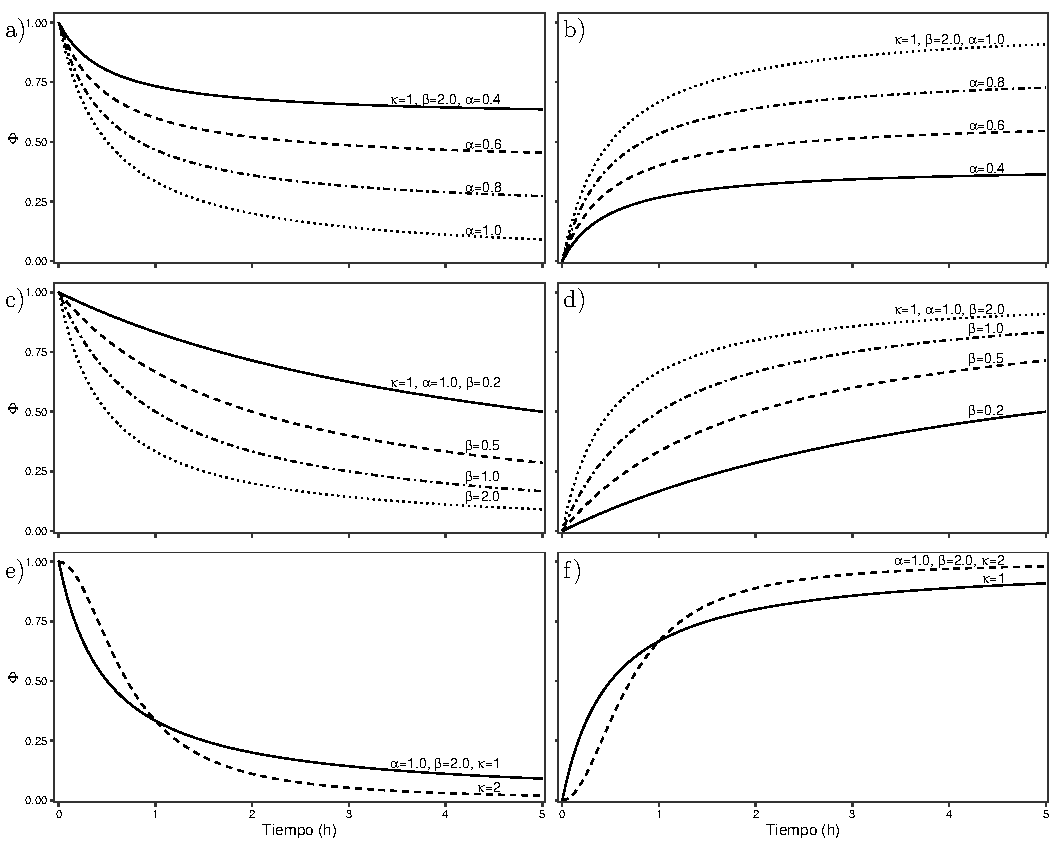
\includegraphics[width = \textwidth]{chap2/images/thesis-models.pdf}
    \caption[Perfiles de transporte simulados con la ecuación propuesta.]{Perfiles de transporte simulados con la ecuación propuesta usando distintos valores de $\alpha$, $\beta$ y $\kappa$ para las disoluciones de alimentación (a., c. y e.) y recuperación (b., d. y f.).}
    \label{fig:Modelssim}
\end{figure}

Puede observarse que para valores de $\beta$ y $\kappa$ constantes (Figuras \ref{fig:Modelssim}(a) y (b)), valores más altos del parámetro $\alpha$ se traducen en valores más pequeños y más grandes para la fracción remanente en la disolución de alimentación y la transportada hacia la disolución de recuperación, respectivamente, para tiempos en los que el sistema ha alcanzado un estado estacionario. 

Cuando los parámetros $\alpha$ y $\kappa$ se mantienen constantes (Figuras \ref{fig:Modelssim}(c) y (d)), los perfiles de transporte que tienden más rápido hacia el estado estacionario presentan valores de $\beta$ más grandes. Para el caso más frecuente en el que $\kappa=1$, el parámetro $\beta$ representa el tiempo al cual la fracción transportada es la mitad de la que será transportada  cuando el sistema alcance el estado estacionario.

Las Figuras \ref{fig:Modelssim}(e) y (f) muestran el cambio en los perfiles de transporte cuando los parámetros $\alpha$ y $\beta$ son constantes, y cambia el parámetro $\kappa$. El comportamiento de las curvas varía principalmente en los primeros momentos del experimento. A pesar de que los parámetros $\alpha$ y $\beta$ son iguales en ambos gráficos, un valor más grande de $\kappa$ produce curvas que llegan más rápido a su valor límite pero que parecen tener un pequeño tiempo de inducción en el que el proceso de transporte se ralentiza. Esto ha sido denominado excentricidad y se ha incluido en la Ecuación \ref{eq:NLSCRIS} para permitir que el modelo abarque un mayor número de sistemas, con un ajuste satisfactorio. Dicho parámetro debe definirse y no debe ser modificado para modelar perfiles de transporte experimentales que hayan sido obtenidos bajo condiciones relativamente similares.


Las ecuaciones que se proponen tienen algunas ventajas respecto a las propuestas en nuestro grupo de investigación hace unos años \citep{RODRIGUEZDESANMIGUEL2014}:
\begin{itemize}
    \item Si el sistema es bien comportado (i.e.\ no hay acumulación significativa de especies en la membrana) los valores de $\alpha$ y $\beta$ son prácticamente iguales para los datos de las disoluciones de alimentación y de recuperación.
    \item Los parámetros $\alpha$ y $\beta$ de cada disolución al ser equivalentes, pueden ser combinados entre sí usando promedios ponderados considerando su respectiva incertidumbre proveniente de la falta de ajuste del modelo \citep{borenstein2011}. Los parámetros obtenidos de esta manera pueden considerarse más robustos y su error asociado es menor.
    \item El número de parámetros que deben ser encontrados por \ac{NLS} es menor. Si el desempeño de dos modelos empíricos es prácticamente el mismo (esto puede ser juzgado por medio de las sumas de los residuales al cuadrado), usualmente se prefiere el más simple.
    \item No hay una combinación posible de parámetros en la que para un tiempo $t=0$, la fracción remanente en la disolución de alimentación sea diferente de uno o la fracción transportada hacia la fase de recuperación sea diferente de cero. Esto es consistente con lo que ocurre en el proceso de extracción.
\end{itemize}   



En el paquete de R \verb|transmem| (ver Capítulo \ref{sec:transmem66i}) se ha incorporado una función para obtener de manera sencilla los parámetros de regresión del modelo propuesto en este trabajo, y también del modelo propuesto por \citet{RODRIGUEZDESANMIGUEL2014}. La función se llama \verb|transTrend()| y su uso se explica en la Sección Anexa \ref{sec:transmemManual}.


\ChapBib{chap2b/chap2b}